\documentclass[conference]{IEEEtran}
\usepackage{amsmath,amssymb,booktabs,graphicx,url,array}
\usepackage[hidelinks]{hyperref}
\graphicspath{{images/}}
\title{Mobility and Assistance-Link Information for Crowd Passage-Time Forecasting: An Exploratory Empirical and Simulation Study}
\author{\IEEEauthorblockN{Surya Maheswaran, Yashaswini Pawar, Sohan Kori, and Seema B. Hegde}
\IEEEauthorblockA{School of Computer Science and Engineering, RV University\\Bengaluru, Karnataka, India}}
\begin{document}
\maketitle
\begin{center}\small\textit{Research Methodology working draft --- 2 November 2026}\end{center}
\begin{abstract}
Mobility differences influence crowd movement, but their physical importance does not establish whether explicit labels improve forecasts beyond observed motion. We examine this distinction through two separate experiments. Eleven recorded SiME bottleneck trials provide 33 observed-cohort prediction checkpoints with three history lengths. Under nested evaluation across width configurations, adding supplied wheelchair information reduces trial-weighted mean absolute error from 4.278 to 2.591 s at the designated one-second history. The benefit varies across configurations and partly reflects crowd composition; artificial label flips can reverse it. A separate prospective synthetic benchmark evaluates helper--client assignment information in a numerically checked JuPedSim escort approximation. In the primary zero-assumed-speed-gain condition, mobility/history and correct-link predictors obtain errors of 0.198 and 0.208 s, respectively. Count and shuffled-link controls also fail to support assignment-specific value. Verified mobility information is therefore useful in the selected empirical sample, while correct assistance links provide no consistent additional forecasting benefit in the tested simulator. Repeated participants, supplied labels, limited layouts and distinct outcomes restrict interpretation. The contribution is an exploratory evaluation of information value and failure modes rather than a validated evacuation-safety system.
\end{abstract}
\begin{IEEEkeywords}assistance relationships, crowd forecasting, heterogeneous mobility, JuPedSim, pedestrian dynamics, SiME\end{IEEEkeywords}

\section{Introduction}
Forecasting crowd passage through bottlenecks requires attention to heterogeneous movement. People differ in mobility, space requirements and interactions with others. SiME provides empirical evidence of such differences in controlled pedestrian settings~\cite{sime,geoerg}. However, an attribute that affects movement need not provide additional predictive information once recent positions and speeds are available.

A wheelchair label may help interpret a short trajectory, or its relevant effect may already be visible in the motion history. Labels can also distinguish different crowd conditions rather than individual movement capacity. Incorrect labels may consequently harm a predictor. Similarly, assistance relationships can govern coordination without necessarily improving forecasts when their explicit endpoints are supplied.

Existing evacuation predictors already use individual characteristics, geometry, speed and congestion~\cite{deng,rset}. Adding these variables or implementing a simulator is not sufficient as a contribution. We instead compare information conditions under matched observations and include controls that challenge the interpretation of apparent improvements.

Two evidence streams address this question. An empirical experiment tests supplied mobility information using recorded SiME trajectories. A separate synthetic experiment evaluates assistance links after numerical checks of a JuPedSim extension. The latter represents circular-agent escorting, not mechanical wheelchair pushing. We retain both positive and negative results and keep their outcome definitions separate.

The practical motivation is to establish which information merits reliable collection before building a forecasting system. The contributions are a matched empirical information comparison, label-quality and composition diagnostics, and a numerically checked assistance prototype with an assignment-control benchmark. Sections II--III establish the literature context, questions and hypotheses; Section IV describes the methods; Sections V--VII present results, interpretation and future work.

\section{Literature Review and Related Work}
\subsection{Search and selection}
The working search was conducted on 2 November 2026 using exploratory web queries and primary publisher, institutional-repository and official dataset/software pages. No publication-year or language filter was applied; sources available by the search date were considered. Targeted checks additionally covered foundational movement, measurement and learning methods; the cited research spans 1970--2024. No authenticated Scopus or Web of Science export was obtained.

Recorded queries included \texttt{evacuation remaining time prediction heterogeneous crowd wheelchair machine learning}, \texttt{"evacuation time prediction" "mobility"}, and \texttt{"remaining evacuation time" prediction wheelchair}. These are the actual search phrases; no uniform database-specific Boolean expression was used. Follow-up searches traced references from the accessible FEMTC paper and checked features, splits and ablations in close forecasting studies.

Inclusion required direct relevance to passage/evacuation prediction, heterogeneous movement, social-group effects or mobility-aid inference, with primary-source evidence. Unrelated navigation, obstacle detection and regional traffic studies were excluded. Normalized titles/DOIs merged duplicate versions. Title/abstract screening and accessible full-text checks produced an initial working register of 15 selected sources, with access status recorded separately. This is not a count of all retrieved hits or 15 fully appraised papers. The expanded manuscript bibliography contains 18 cited references, including foundational methods, software and a dataset; this is not a count of PRISMA-included empirical studies. Historical PRISMA counts are not reused for this revised question, and no completed systematic-review flow is claimed.

\subsection{Critical comparison and synthesis}
SiME studies movement of heterogeneous populations through controlled facilities. Geoerg et al.~\cite{geoerg} examine individual impairments and crowd-flow relations, while subsequent work~\cite{sime} analyses bottleneck movement, neighbourhoods and behaviour. These findings motivate mobility-aware analysis, but do not by themselves establish the incremental predictive value of a supplied label for our target.

Published measurement definitions are important. Reliable trajectory extraction is a distinct measurement task~\cite{boltes}; Voronoi-based measurement reduces scatter in local crowd quantities~\cite{steffen}. SiME's bottleneck analysis uses Voronoi speed aggregation, Delaunay neighbours and specified observation intervals~\cite{sime}. Our development diagnostics use displacement speeds and nearest visible-track spacing. They are not exact replications of those published procedures. Downstream head-centre passage is also distinct from bottleneck-entry flow.

Deng et al.~\cite{deng} introduce an evacuation-time predictor using individual characteristics and congestion information with simulation-based targets. Uhl\'{i}k et al.~\cite{rset} compare evacuation surrogates across geometries. Their related complex-geometry study~\cite{femtc} provides a concrete methods example using count, distance, spacing and walking-speed summaries. These precedents rule out broad claims of first incorporating individual characteristics or movement speed.

JuPedSim provides microscopic operational models and direct-steering interfaces~\cite{jps}. Targets can be changed while retaining operational interactions. This software capability does not empirically validate assistance rules or wheelchair representations. We distinguish implementation verification, numerical sensitivity and behavioural validation.

Microscopic movement also has established alternatives. The Social Force Model represents desired motion and interactions through force terms~\cite{helbing}; the Optimal Steps Model selects discrete movement steps in continuous space~\cite{seitz}. Collision-free speed modelling relates pace to available space, agent size and time gap~\cite{tordeux}. Our implementation uses JuPedSim's documented speed-model variant, not the Social Force or Optimal Steps Model. These models explain operational movement and do not by themselves establish that labels improve a learned forecast.

Moussa\"id et al.~\cite{moussaid} show that social groups exhibit characteristic formations and movement effects. This supports studying relationships but does not calibrate wheelchair assistance: a social group is not necessarily a helper--client pair. Likewise, a physical effect of coordination does not demonstrate incremental predictive value once observed motion is known. Explicit assignment controls are therefore needed.

The review is a bounded scoping investigation with recorded queries and access limitations. Some closest temporal-prediction and scene-assessment papers remain incompletely accessible for full feature, split and ablation extraction. We claim neither exhaustive coverage nor first-of-its-kind novelty. The study contributes a qualified information comparison and documented failure modes.

Table~\ref{tab:literature} summarizes the directly used research. Together these studies establish heterogeneous movement and speed-aware prediction as prior art. The narrower unresolved question addressed here is whether explicit mobility or assignment information improves the specified forecast beyond matched observed-motion inputs. This is an operational evaluation question, not proof that prior literature has never tested related features.

\begin{table*}[t]
\caption{Comparative literature matrix for the directly used research. Access limitations restrict claims about absent methods.}\label{tab:literature}
\centering\footnotesize\setlength{\tabcolsep}{4pt}
\begin{tabular}{>{\raggedright\arraybackslash}p{0.12\textwidth}>{\raggedright\arraybackslash}p{0.14\textwidth}>{\raggedright\arraybackslash}p{0.15\textwidth}>{\raggedright\arraybackslash}p{0.14\textwidth}>{\raggedright\arraybackslash}p{0.16\textwidth}>{\raggedright\arraybackslash}p{0.16\textwidth}}
\toprule Author/year & Objective & Methodology & Dataset/sample & Key finding or contribution & Limitation for this question\\\midrule
Geoerg et al., 2022~\cite{sime} & Explain disability-related bottleneck movement & Controlled trajectory and neighbourhood analysis & Heterogeneous SiME bottleneck trials & Empirical differences in movement and interactions & Does not establish incremental forecast value for our target\\
Geoerg et al., 2021~\cite{geoerg} & Examine impairments in crowd dynamics & Empirical crowd-flow analysis & Controlled mixed-mobility experiments & Documents impairment-related movement effects & Movement effects alone do not quantify forecast gain\\
Deng et al., 2022~\cite{deng} & Estimate building evacuation time & Predictor using individual characteristics and congestion & Simulation-based evacuation outcomes & Establishes individual/congestion-aware prediction as prior art & Different outcome; full feature/split extraction remains incomplete\\
Uhl\'{i}k et al., 2024~\cite{rset} & Compare RSET surrogates across geometries & Comparative machine-learning evaluation & Simulation training datasets, three geometry types & Establishes geometry-aware surrogate comparison & Published metrics are not directly comparable to our cohort target\\
Uhl\'{i}k, 2024~\cite{femtc} & Predict RSET in a complex geometry & Simulation-trained machine learning & Complex-geometry simulation case & Uses count, distance, spacing and speed summaries & Does not validate our real-data target or escort mechanism\\\bottomrule
\end{tabular}
\end{table*}

\section{Research Problem, Objectives and Hypotheses}
The empirical question is whether explicit wheelchair information improves remaining-passage forecasts beyond recent movement and geometry summaries. The synthetic question is whether correct helper--client assignments add value beyond individual mobility/history and assistance-link counts.

Our objectives are to define past-only inputs and observed outcomes; compare information conditions under grouped evaluation; quantify label-error sensitivity; and test assistance-link value without assuming that assistance increases movement speed. Labels and links are supplied, not automatically recognized.

\textbf{RQ1:} Does supplied mobility information improve observed-cohort passage-time prediction beyond motion and geometry? \textbf{RQ2:} How do history length, label quality and crowd composition qualify that improvement? \textbf{RQ3:} In the separate escort approximation, do correct assignments outperform mobility/history, count-only and shuffled-link conditions?

\textbf{H1:} mobility information reduces empirical trial-weighted error at the primary one-second history. The null direction is no reduction or increased error. \textbf{H2:} the mobility benefit is greater with shorter histories. \textbf{H3:} correct assistance links reduce synthetic error beyond mobility/history under zero assumed speed gain. Correct links must also outperform count-only and shuffled-link controls to support assignment-specific value.

Let $D_E(h)=\operatorname{MAE}(H,h)-\operatorname{MAE}(M,h)$. For H1, $H_{0,E}:D_E(1)\leq0$ and $H_{1,E}:D_E(1)>0$ describe directional evaluation criteria. H2 requires gains to decrease as history increases over 0.4, 1 and 2 s. For H3, $H_{0,S}:\Delta\leq0$ versus $H_{1,S}:\Delta>0$, additionally subject to the two assignment controls. These are exploratory operational hypotheses; no population-level null rejection is claimed.

The independent information variables are feature condition, history length and artificial label/edge availability. The dependent outcomes are forecast errors against the separately defined empirical and synthetic times. Matched cohorts, checkpoints, folds and learner grids control comparisons; synthetic block geometry and sampled paces are matched across modes. Repeated identities, population composition, coupled widths and unmeasured behaviour remain potential confounds. Wheelchair membership means the documented source classification, not a medical inference from speed.

The empirical outcomes were inspected during development before evaluation design. The synthetic protocol, scenarios and implementation were hashed before new benchmark outcomes, but the movement model had undergone adaptive development. These qualifications prevent a population-level confirmatory interpretation.

\section{Research Methodology}
\subsection{Research design and procedure}
This quantitative comparative study adopts a pragmatic position: information is assessed by its measured utility for a stated prediction task. Secondary observational trajectories provide exploratory empirical evidence; controlled computational experiments test assignment information within a specified generator. Neither component estimates a causal human assistance effect. Figure~\ref{fig:workflow} summarizes the research procedure.

\begin{figure}[t]
\centering\small
\fbox{\begin{minipage}{0.92\columnwidth}\centering
Problem and literature review\\$\downarrow$\\
Gap, objectives, questions and hypotheses\\$\downarrow$\\
Select design, eligible data and outcome definitions\\$\downarrow$\\
Audit trajectories / implement and verify escort model\\$\downarrow$\\
Extract past-only features; define grouped partitions\\$\downarrow$\\
Fit on training data; select on validation data\\$\downarrow$\\
Evaluate baselines, labels, links and controls\\$\downarrow$\\
Reconstruct results; interpret limits and conclusions
\end{minipage}}
\caption{Research procedure. Empirical outcomes were exposed during development; synthetic benchmark samples followed the frozen protocol.}\label{fig:workflow}
\end{figure}

\subsection{Empirical data and target}
We reuse the SiME trajectory archive~\cite{dataset}. The primary set contains seven complete wheelchair-containing trials (501--506 and 508) and four reference trials (1501, 1503, 1505 and 1507), spanning widths of 0.9--1.2 m. Seven documented wheelchair users repeat across trials. Positions are recorded at 25 Hz. Track counts, internal continuity, header mappings and downstream crossings were audited.

Trial 507 is excluded from the primary bundle because one wheelchair track ends before the measurement line. Trial 1307 has inconsistent metadata/track counts, while 1301 lies outside the currently verified primary class scope. Their diagnostic records are retained. Difficult individuals are not deleted to manufacture complete targets.

Selection is purposive from available, audited archive trials, not random sampling of public crowds. Fourteen trial files were audited and eleven met the primary completeness/class criteria. Sample size follows those eligibility constraints; no power calculation or population-representativeness claim is made. Local source identity and file integrity were checked against saved provenance and archive checksums; the current audit and six-file acquisition are dated 2 November 2026. Raw tracks remain local because current redistribution conditions have not been established.

At recording time $t\in\{10,20,30\}$ s, let $C(t)$ contain currently visible tracks upstream of $x=2.4$ m with continuous observations over $[t-2,t]$. The same cohort is used for 0.4, 1 and 2 s histories. Thus even the shortest-history experiment is conditional on two-second track availability. With $\tau_i$ the first forward head-centre crossing, interpolated between adjacent frames, the target is
\begin{equation}Y_E(t)=\max_{i\in C(t)}\tau_i-t.\end{equation}
Later arrivals are excluded. Missing member crossings make the cohort target incomplete. This measures an observed subset's passage, not whole-building evacuation or full-body clearance. The bundle contains 33 query cohorts and 99 correlated history rows.

\subsection{Features, models and evaluation}
Condition H contains 19 summaries: active count; x/y means and spreads; distance mean, maximum and 90th percentile; speed mean, spread, 10th and 90th percentiles; stopped fraction; speed change; nearest visible spacing; past crossings; elapsed time; and bottleneck/corridor widths. Backward displacement stays inside each selected history. The stopped threshold is 0.1 m/s.

M adds wheelchair count, fraction, group mean observed speed, group maximum distance and presence. Empty-group values are zero. The selected conditions use documented wheelchair IDs and source metadata; no age, family or helper graph is inferred. Supplied labels represent a reference information condition, not detector outputs.

Four outer folds omit all trials at one width configuration. Inner folds omit one of the remaining widths for selection. Separating tuning from error estimation addresses selection bias~\cite{varma}; grouping observations addresses dependence~\cite{roberts}. Queries and histories from a trial stay together. Because participants repeat, this is transfer across configurations within a shared population. Corridor width, crowd size and composition also vary; the design does not isolate a causal doorway-width effect.

Ridge regression~\cite{hoerl} regularizes correlated summaries; gradient boosting~\cite{friedman} provides a nonlinear tree-based comparison. Ridge penalties are $\{0.1,1,10,100\}$. Boosting uses learning rates $\{0.03,0.1\}$, depths $\{2,3\}$ and 50/100 estimators, with seed 113. Scaling is fitted inside training partitions; validation selects settings with deterministic ties. Predictions are clipped below at zero. Training-median and simple distance/speed estimates are references. We report matched-family and validation-selected results.

The primary metric averages query errors within each trial, then trials equally:
\begin{equation}\operatorname{MAE}=\frac1R\sum_{r=1}^R\frac1{Q_r}\sum_{q=1}^{Q_r}|\widehat Y_{rq}-Y_{rq}|.\end{equation}
Frames, history versions and artificial masks are not independent participants.

No missing target is imputed and no target-based outlier trimming is performed. Eligible feature values are checked for finiteness; zero-filled absent groups are defined encodings rather than estimated missing measurements. Duplicate keys and invalid trajectories are audited before fitting. Numerical processing uses NumPy 2.3.5, model fitting scikit-learn 1.7.2~\cite{sklearn}, plotting Matplotlib 3.11.2, and synthetic geometry Shapely 2.1.2. The study runs locally in Python; hardware throughput is not an evaluated outcome. Version pins, feature manifests, selection traces and saved predictions support reproduction.

Analysis is descriptive: absolute MAE differences, relative error reduction, bias, worst-trial error and width/trial breakdowns are reported. MAE expresses timing error directly in seconds without treating a few large errors as squared losses. Mask variability is a deterministic stress range, not a confidence interval. No inferential test, significance threshold, degrees of freedom or population confidence interval is specified; outcome-informed empirical development, repeated participants and few grouped configurations make confirmatory significance claims inappropriate. Directional hypothesis assessments therefore concern these saved evaluations only.

\subsection{Label and composition follow-ups}
After the initial comparison, fixed clean-trained models receive label unavailability probabilities of 0.25/0.50/0.75 or symmetric binary-flip probabilities of 0.10/0.25. Twenty deterministic masks are shared across each trial's checkpoints. Unavailable labels contribute no positive membership while the full cohort denominator is retained. No missingness indicator or uncertainty-aware retraining is introduced. These are artificial errors, not measured recognition performance.

Composition ablations add presence alone, count/fraction/presence, or labelled-group speed/distance. Anonymous-motion additions comprise rearmost observed speed, minimum person speed and maximum distance/speed estimates with fixed denominator floors. These post-result development comparisons use the original nested design. Their best evaluation result does not replace the initial headline.

\subsection{Synthetic escort approximation}
The separate JuPedSim 1.4.2 extension uses CollisionFreeSpeedModelV2 with neighbour-repulsion strength 2.6. Client/helper circular radii are 0.30/0.22 m. Helpers have a 0.3 s native time gap; others use 0.8 s. Native routing/interactions move agents; positions are never overwritten.

The helper targets the client's current position and waits below 0.70 m separation. The client waits above 1.2 m and resumes below 1.0 m. Coordinated client pace is $\min(gv_c,v_h)$ for nominal paces $v_c,v_h$. Primary gain $g=1$ avoids programming faster assistance; $g=1.15$ is secondary. Each person exits only after its full nominal circle crosses the plane. A remaining helper completes its own exit after the client leaves.

This controller has no push contact, force transmission, wheel kinematics or elongated wheelchair footprint. A numerically reliable parameter is not necessarily an empirically realistic one. Earlier failures remain preserved. The selected configuration passed twelve development fixtures covering doors, turns, multiple pairs and perturbed queues. Checks cover finite positions, counts, circle overlap $\leq0.001$ m, wall penetration $\leq0.005$ m, speed ceilings and pair gaps. Timing tolerance is $\max(0.2\text{ s},1\%$ of finer clearance$)$.

\subsection{Frozen synthetic experiment}
Four layouts contain two serial pairs through 1.0/1.2 m doors, a staggered merge and a turn. Twelve seeds per layout draw client paces in $[0.70,0.95]$ m/s, helper paces in $[1.1,1.3]$ m/s and pairwise lateral offsets in $[-0.02,0.02]$ m. Matched independent/coordinated modes at both gains give 192 main runs from 48 blocks. Slots 0--7 train, 8--9 validate and 10--11 evaluate. Layouts appear in all partitions; this tests new sampled blocks within known layouts.

All main runs at 0.005 s and 48 predetermined finer replays at 0.0025 s passed admission; maximum clearance difference was 0.005 s. No failed run was dropped or redrawn. Queries at 2/5/8 s use one second of past snapshots and target remaining time to the last full-circle crossing of the known roster. All 576 queries were eligible. This target differs from empirical head-centre passage for an observed subset.

Synthetic M contains 31 history, geometry and supplied-mobility summaries, including nominal pace/radius, role counts and distance/nominal-pace estimates. It excludes links, waiting states, gain labels and IDs. F-counts adds active-link count and linked-client fraction. F-correct adds pair gaps, speed differences, helper-minus-client nominal pace and route separation. F-shuffled swaps the two helper assignments, preserving initial endpoint degrees. Empty-edge summaries are zero. F-missing withholds each edge with probability 0.5 in a deployment-only 20-mask stress.

Each coordinated gain stratum has 32/8/8 train/validation/evaluation runs. The empirical ridge/boosting grid is reused; training-only fits and validation selection precede evaluation. No train-plus-validation refit occurs. Primary contrast is $\Delta=\operatorname{MAE}(M)-\operatorname{MAE}(F_{\rm correct})$ at zero gain. We report run/layout results without population-significance claims.

\section{Results}
\subsection{Empirical comparison}
At one-second history, M reduces MAE from 4.278 to 2.591 s, a 1.687 s or 39.4\% aggregate reduction (Table~\ref{tab:emp}). Ridge is selected in all four primary folds for H and M. Bias changes from $+0.560$ to $-0.068$ s; worst-trial MAE from 6.999 to 5.549 s. This supports H1's direction in the sample without establishing population significance.

\begin{table}[t]\caption{Initial empirical equal-trial errors (s).}\label{tab:emp}\centering
\begin{tabular}{lrr}\toprule Model/history&H&M\\\midrule
Selected, 0.4 s&4.034&2.785\\
Selected, 1 s (primary)&4.278&2.591\\
Selected, 2 s&4.121&2.591\\
Matched boosting, 1 s&9.181&6.703\\\bottomrule\end{tabular}\end{table}

M improves in eight of eleven trials, but worsens at the 1.2 m configuration (Fig.~\ref{fig:width}), which contains two selected trials. Training-median and simple travel-time errors are 18.594/24.102 s at the primary history. These weak references do not represent every analytical evacuation model. The mobility gain is not monotonically larger with shorter histories, leaving H2 unsupported as stated.

\begin{figure}[t]\centering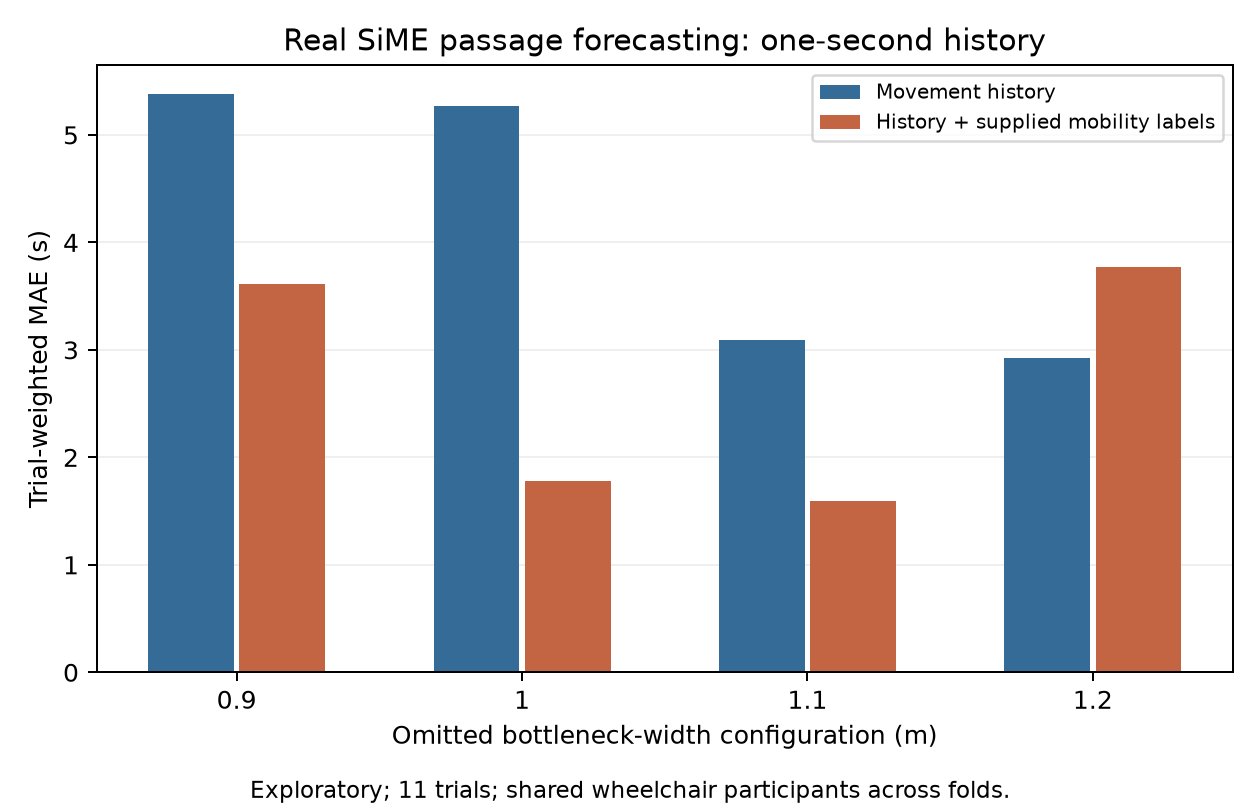
\includegraphics[width=\columnwidth]{empirical_width.png}\caption{Primary empirical errors by omitted width configuration. Participants repeat, and geometry/population conditions differ across configurations.}\label{fig:width}\end{figure}

\subsection{Label quality and composition}
Missing-label fallback retains some benefit on average; symmetric flips sharply increase errors (Table~\ref{tab:noise}). The slight improvement at 25\% unavailability is a finite-sample response, not a recommendation to hide information. Mask ranges are not population confidence intervals.

\begin{table}[t]\caption{Fixed-model empirical label stress.}\label{tab:noise}\centering
\begin{tabular}{lrr}\toprule Error probability&Mean MAE (s)&Mask range (s)\\\midrule
Unavailable, 0.25&2.517&2.226--2.939\\
Unavailable, 0.50&2.674&2.322--3.649\\
Unavailable, 0.75&3.782&2.570--5.463\\
Flip, 0.10&8.148&7.628--8.730\\
Flip, 0.25&11.437&10.550--12.094\\\bottomrule\end{tabular}\end{table}

Presence alone gives 3.190 s MAE; counts/fraction/presence gives 3.231 s. Labelled-group speed/position gives 2.443 s in the follow-up. Anonymous additions give 4.650 s, or 3.054 s with full M. More features do not automatically produce a stronger baseline; the follow-up winner does not replace the original 2.591 s result.

Composition explains a substantial predictive difference, not a causal proportion of delay. In models trained on both conditions, full M reduces wheelchair-trial MAE from 4.007 to 2.921 s and reference-trial MAE from 4.753 to 2.015 s. Reference improvements reinforce that crowd-condition identification can contribute to the gain.

\subsection{Synthetic assistance links}
At zero gain, correct links yield $\Delta=-0.009305$ s: slightly higher error than M (Table~\ref{tab:links}). They also fail to outperform count and shuffled controls. H3 is unsupported in this benchmark. Wrong links are not selected as a desirable system based on these evaluation scores.

\begin{table}[t]\caption{Synthetic selected-model MAE (s); eight evaluation runs and 24 queries per gain.}\label{tab:links}\centering
\begin{tabular}{lrr}\toprule Information&$g=1$ (primary)&$g=1.15$\\\midrule
Mobility/history M&0.198&0.200\\
F-counts&0.198&0.200\\
F-correct&0.208&0.263\\
F-shuffled&0.182&0.177\\
F-missing, mask mean&0.318&0.268\\\bottomrule\end{tabular}\end{table}

All primary conditions select ridge penalty 0.1. Matched boosting changes from 0.329 to 0.319 s with correct links, while shuffled boosting reaches 0.313 s; this does not reverse the selected-model interpretation. At gain 1.15, M selects ridge and F-correct boosting, again without a consistent correct-link advantage.

All coordinated query graphs retain two active links, including shuffled graphs; counts are constant and effectively uninformative. Wrong-link summaries may act as other spatial descriptors. Their lower errors do not imply that physically assigning the wrong helper improves clearance. Exact nominal paces and simple layouts make M a strong predictor of this generator.

Median/travel-time references give 2.419/1.018 s at zero gain. F-missing errors average 0.318 s (mask range 0.200--0.437 s) and 0.268 s (0.230--0.299 s) across gains. Coordinated-minus-independent movement clearance averages $+0.279$ s at zero gain and $-1.771$ s at gain 1.15 over all blocks. The latter contains a programmed benefit and is not evidence of real assistance effectiveness.

\subsection{Verification}
Independent saved-output reconstruction verifies 792 initial empirical, 3,300 label-stress, 231 composition-check and 1,632 synthetic predictions. Checks cover unique keys, target reconstruction, denominators and evaluation membership. Feature checks remove future frames: 99 original empirical, 33 anonymous-summary and 1,152 synthetic correct/shuffled checks pass. Hashes and full selection traces are retained. These audits do not independently reimplement every learner or integration-step geometry calculation.

\section{Discussion}
The evidence separates three propositions: mobility affects movement; supplied mobility can improve a forecast; and correct assistance assignments add further predictive value. The first motivates the study, the second receives limited empirical support, and the third is unsupported by the selected synthetic features and learners.

This is consistent with SiME's evidence that heterogeneous movement deserves explicit attention~\cite{sime,geoerg}, but extends neither its population scope nor its behavioural validation. Deng's characteristic-aware predictor and the RSET surrogate studies~\cite{deng,rset,femtc} establish relevant precedent; different targets and evaluation populations prevent direct ranking against their reported errors. The present contribution lies in matched information controls and qualified interpretation of their outcomes.

Empirical labels partly identify populations with different counts and behaviour. The same seven wheelchair users appear across configurations, and zero-default group summaries encode presence. Independent populations or controlled composition variation would be needed to isolate individual mobility effects. A 39.4\% sample-level reduction should not be interpreted as general expected improvement.

False positives can create numerous spurious memberships when the positive class is sparse, including in reference crowds. A recognition module would need class-specific precision/recall, calibration, an unknown state and downstream forecast testing. No such detector is trained here; artificial error probabilities cannot replace its evaluation.

The synthetic negative finding is informative within a constrained generator. Early observations, fixed pair counts, supplied nominal paces, two pairs and limited layouts may leave little residual information for an explicit graph. Other mechanisms could matter, but adding delays or hidden states solely to make correct links win would undermine the comparison. Any extension requires independent justification and a new protocol.

The empirical design is exploratory because outcomes informed development; the synthetic design is prospective only relative to its new samples. Repeated people and matched variants limit effective sample sizes. No operational tolerance or population significance is established. Exact reproduction of published SiME measurements and exhaustive closest-paper coverage remain incomplete.

The targets also differ: empirical head-centre passage for an observed subset versus complete-roster synthetic circle clearance. Neither represents alarm-to-safety, and their MAEs cannot be pooled to suggest superior real-world simulation accuracy. Physical pushing, age effects and family relationships remain outside the evaluated scope. Public-data terms and final author declarations need verification before submission.

\section{Conclusion and Future Work}
Supplied mobility information reduces primary aggregate error from 4.278 to 2.591 s in eleven selected SiME trials. Composition controls and label-error tests qualify that result: condition information contributes, and incorrect labels can erase the benefit. In a separate numerically checked escort benchmark, correct helper assignments show no consistent improvement beyond mobility/history, counts and shuffled controls. Both outcomes are retained.

Future work should prioritize independent participants/layouts, controlled composition differences and calibrated label uncertainty. Empirical helper identities and coordination measurements are needed for behavioural validation. Physical wheelchair pushing requires suitable footprints and contact mechanics beyond circular escorts. The current study supports a cautious information-value evaluation, not an operational evacuation-safety claim.

\section*{Research Declarations}
No external funding was reported. No new human participants were recruited; public SiME trajectories are reused with credit to their investigators. Only coded source identities are used; raw trajectories and mappings remain local and are not redistributed. Secondary reuse does not establish a new consent or ethics exemption: applicable institutional permission and source terms require confirmation before submission. Synthetic runs are separately identified. AI tools assisted coding and manuscript preparation; authors remain responsible for verification. Author spellings, affiliation details, institutional emails, contributions, conflicts and institutional data-use declarations require author confirmation.

\begin{thebibliography}{18}
\bibitem{sime} P. Geoerg, J. Schumann, M. Boltes, and M. Kinateder, ``How people with disabilities influence crowd dynamics of pedestrian movement through bottlenecks,'' \textit{Scientific Reports}, vol. 12, art. 14273, 2022, doi: 10.1038/s41598-022-18142-7.
\bibitem{geoerg} P. Geoerg, J. Schumann, S. Holl, and M. Boltes, ``The influence of individual impairments in crowd dynamics,'' \textit{Fire and Materials}, vol. 45, no. 4, pp. 529--542, 2021, doi: 10.1002/fam.2789.
\bibitem{deng} Q. Deng et al., ``Evacuation time estimation model in large buildings based on individual characteristics and real-time congestion situation of evacuation exit,'' \textit{Fire}, vol. 5, no. 6, art. 204, 2022, doi: 10.3390/fire5060204.
\bibitem{rset} O. Uhl\'{i}k, P. Ok\v{r}inov\'{a}, A. Tokarevskikh, T. Apeltauer, and J. Apeltauer, ``Real-time RSET prediction across three types of geometries and simulation training dataset: A comparative study of machine learning models,'' \textit{Developments in the Built Environment}, vol. 18, art. 100461, 2024, doi: 10.1016/j.dibe.2024.100461.
\bibitem{boltes} M. Boltes and A. Seyfried, ``Collecting pedestrian trajectories,'' \textit{Neurocomputing}, vol. 100, pp. 127--133, 2013, doi: 10.1016/j.neucom.2012.01.036.
\bibitem{steffen} B. Steffen and A. Seyfried, ``Methods for measuring pedestrian density, flow, speed and direction with minimal scatter,'' \textit{Physica A}, vol. 389, no. 9, pp. 1902--1910, 2010, doi: 10.1016/j.physa.2009.12.015.
\bibitem{femtc} O. Uhl\'{i}k, ``Real-time RSET prediction based on simulation dataset using machine learning: A complex geometry case study,'' in \textit{Fire and Evacuation Modeling Technical Conference}, 2024. [Online]. Available: \url{https://files.thunderheadeng.com/femtc/2024_d1-03-uhlik-paper.pdf}
\bibitem{jps} JuPedSim developers, ``JuPedSim 1.4.2: API reference and routing documentation.'' [Online]. Available: \url{https://www.jupedsim.org/v1.4.2/}. Accessed: Nov. 2, 2026.
\bibitem{helbing} D. Helbing and P. Moln\'{a}r, ``Social force model for pedestrian dynamics,'' \textit{Physical Review E}, vol. 51, no. 5, pp. 4282--4286, 1995, doi: 10.1103/PhysRevE.51.4282.
\bibitem{seitz} M. J. Seitz and G. K\"oster, ``Natural discretization of pedestrian movement in continuous space,'' \textit{Physical Review E}, vol. 86, art. 046108, 2012, doi: 10.1103/PhysRevE.86.046108.
\bibitem{tordeux} A. Tordeux, M. Chraibi, and A. Seyfried, ``Collision-free speed model for pedestrian dynamics,'' in \textit{Traffic and Granular Flow '15}, Cham, Switzerland: Springer, 2016, pp. 225--232, doi: 10.1007/978-3-319-33482-0\_29.
\bibitem{moussaid} M. Moussa\"id, N. Perozo, S. Garnier, D. Helbing, and G. Theraulaz, ``The walking behaviour of pedestrian social groups and its impact on crowd dynamics,'' \textit{PLOS ONE}, vol. 5, no. 4, art. e10047, 2010, doi: 10.1371/journal.pone.0010047.
\bibitem{dataset} P. Geoerg, M. Boltes, S. Holl, D. Salden, and J. Schumann, ``Influence of individual characteristics,'' \textit{Pedestrian Dynamics Data Archive}, dataset, doi: 10.34735/ped.2017.1.
\bibitem{varma} S. Varma and R. Simon, ``Bias in error estimation when using cross-validation for model selection,'' \textit{BMC Bioinformatics}, vol. 7, art. 91, 2006, doi: 10.1186/1471-2105-7-91.
\bibitem{roberts} D. R. Roberts et al., ``Cross-validation strategies for data with temporal, spatial, hierarchical, or phylogenetic structure,'' \textit{Ecography}, vol. 40, no. 8, pp. 913--929, 2017, doi: 10.1111/ecog.02881.
\bibitem{hoerl} A. E. Hoerl and R. W. Kennard, ``Ridge regression: Biased estimation for nonorthogonal problems,'' \textit{Technometrics}, vol. 12, no. 1, pp. 55--67, 1970, doi: 10.1080/00401706.1970.10488634.
\bibitem{friedman} J. H. Friedman, ``Greedy function approximation: A gradient boosting machine,'' \textit{The Annals of Statistics}, vol. 29, no. 5, pp. 1189--1232, 2001, doi: 10.1214/aos/1013203451.
\bibitem{sklearn} F. Pedregosa et al., ``Scikit-learn: Machine learning in Python,'' \textit{Journal of Machine Learning Research}, vol. 12, pp. 2825--2830, 2011. [Online]. Available: \url{https://jmlr.org/papers/v12/pedregosa11a.html}
\end{thebibliography}
\end{document}

